\documentclass[t]{beamer}
   \usepackage{bm,amssymb, amsmath, graphicx}
   \usepackage{booktabs}
   \usepackage{caption}
\usepackage{subcaption}
\usepackage{float}
\usepackage{mathrsfs}
\usepackage{array} 
\usepackage{rotating}
\usepackage{rotating}
 \providecommand{\abs}[1]{\lvert#1\rvert}
\providecommand{\norm}[1]{\lVert#1\rVert}
 \usetheme{Boadilla}
 \usefonttheme[onlymath]{serif}
 \setbeamertemplate{blocks}[rounded][shadow=false]
 \setbeamertemplate{navigation symbols}{}


 \title[The Joint Graphical Lasso]{The Joint Graphical Lasso for \\Inverse Covariance Estimation Across Multiple Classes}
 \subtitle{P. Danaher, P. Wang \& D. Witten}
 \author[Abrahamsen \& Rahman]{Tavis Abrahamsen \\ Syed Rahman}
 \institute[ ]{Department of Statistics \\ University of Florida}
\date{April 16, 2015}
\begin{document}



\begin{frame}
 \titlepage
\end{frame}

\begin{frame}
\frametitle{Background}
Suppose that observations $\bm{x}_{1},\bm{x}_{2},\ldots,\bm{x}_{n} \in \mathbb{R}^{P}$ are independent and identically distributed $N(\bm{\mu},\bm{\Sigma})$ where $\bm{\mu} \in \mathbb{R}^{p}$ and $\bm{\Sigma}$ is a positive definite $p\times p$ matrix. 

\bigskip
\pause
The zeros in the inverse covariance matrix $\bm{\Sigma}^{-1}$ correspond to pairs of features that are conditionally independent - that is, pairs of variables that are independent of each other, given all the other variables in the data set.

\bigskip
\pause
In a Gaussian graphical model, the conditional dependence relationships are represented by a graph in which nodes represent the features and edges connect conditionally dependent pairs of features.
\end{frame}

\begin{frame}
\frametitle{Background}
A natural way to estimate the precision (or concentration) matrix $\bm{\Sigma}^{-1}$ is via maximum likelihood.  Letting $\bm{S}$ denote the empirical covariance matrix of $X$, the Gaussian log likelihood takes the form (up to a constant)
\small
\begin{equation*}
\frac{n}{2}\log\, \det \bm{\Sigma}^{-1} - \mbox{trace}\left(\bm{S\,\Sigma}^{-1}\right)
\end{equation*}

\normalsize
\bigskip
\pause
Maximizing this function with respect to $\bm{\Sigma}^{-1}$ yields the maximum likelihood estimate $S^{-1}$.

\bigskip
\pause
Problems with using the MLE of $\bm{\Sigma}^{-1}$:
\begin{itemize}
	\item[1.] In the high dimensional setting where $p > n$ the matrix $\bm{S}$ is singular and cannot be inverted to yield an estimate of $\bm{\Sigma}^{-1}$.
	
	\bigskip
	\item[2.] Even when $\bm{S}^{-1}$ exists, this estimator will typically not be sparse.
\end{itemize}
\end{frame}


\begin{frame}
\frametitle{Background}
One method for obtaining sparse estimates of $\bm{\Sigma}^{-1}$ is to instead solve the \textit{graphical lasso} problem
\small
\begin{equation*}
\max_{\bm{\Theta}} \log\,\det \bm{\Theta} - \mbox{trace}\left(\bm{S \,\Theta}\right) - \lambda ||\bm{\Theta}||_{1},
\end{equation*}
\normalsize
where $\lambda$ is a nonnegative tuning parameter. 



\bigskip
\pause
Advantages of using the graphical lasso estimator:
\begin{itemize}
\item[1.]  The $l_{1}$ penalty term yields sparse estimates of $\bm{\Sigma^{-1}}$ when $\lambda$ is ``large".

\bigskip
\item[2.] This problem can be solved even if $p \gg n$.
\end{itemize}
\end{frame}

\begin{frame}
\frametitle{Motivation - Genetics}
Graphical models are of particular interest in the analysis of gene expression data since they can provide a useful tool for visualizing the relationships among genes and generating biological hypotheses.

\bigskip
\pause
The standard formulation for estimating a Gaussian graphical model assumes that each observation is drawn from the same distribution. However, in many datasets the observations may correspond to several distinct classes.

\bigskip
\pause
For example, suppose a cancer researcher collects gene expression measurements for a set of cancer tissue samples and a set of normal tissue samples.  One might want to estimate a graphical model for the cancer samples and a graphical model for the normal samples.

\bigskip
\pause
One might expect the two graphical models to be similar to each other since both are based on the same type of tissue, but also have important differences resulting from the fact that gene networks are often dysregulated in cancer.

\end{frame}

\begin{frame}
\frametitle{The Joint Graphical Lasso}
The authors propose the \textit{joint graphical lasso} as a technique for jointly estimating multiple graphical models corresponding to distinct but related conditions, such as cancer and normal tissue.

\bigskip
\pause
Suppose we have data from $K \geq 2$ distinct classes.  Instead of estimating $\bm{\Sigma}_{1}^{-1},\bm{\Sigma}_{2}^{-1},\ldots,\bm{\Sigma}_{K}^{-1}$ separately, the authors propose estimating estimating these values jointly by maximizing the following penalized log-likelihood function
\small
\begin{equation*}
\max_{\{\bm{\Theta}\}} \sum_{k=1}^{K}n_{k}\left[\log\,\det \bm{\Theta}^{(k)}-\mbox{trace}\left(\bm{S}^{(k)}\bm{\Theta}^{(k)}\right)\right] - P(\{\bm{\Theta}\}),
\end{equation*}
\normalsize
subject to the constraint that $\bm{\Theta}^{(1)},\bm{\Theta}^{(2)},\ldots,\bm{\Theta}^{(K)}$ are positive definite, where $\{\bm{\Theta}\} = \{\bm{\Theta}^{(1)},\bm{\Theta}^{(2)},\ldots,\bm{\Theta}^{(k)}\}$.

\bigskip
\pause
$P(\{\bm{\Theta}\})$ denotes a convex penalty function, so the objective function is strictly concave.
\end{frame}

\begin{frame}
\frametitle{Joint Graphical Lasso}
The authors propose choosing a penalty function $P$ that will encourage $\hat{\bm{\Theta}}^{(1)},\hat{\bm{\Theta}}^{(2)},\ldots,\hat{\bm{\Theta}}^{(K)}$ to share certain characteristics, such as the locations or values of the nonzero elements, in addition to providing sparse estimates of the precision matrices.

\bigskip
\pause
Two penalty functions suggested by the authors are the \textit{fused graphical lasso} and \textit{group graphical lasso} penalties.
\end{frame}

\begin{frame}
\frametitle{Fused Graphical Lasso}
The fused graphical lasso (FGL) penalty is given by
\small
\begin{equation*}
P(\{\bm{\Theta}\}) = \lambda_{1}\sum_{k=1}^{k}\sum_{i\neq j}|\theta_{ij}|^{(k)} + \lambda_{2}\sum_{k<k'}\sum_{i,j}|\theta_{ij}^{(k)}-\theta_{ij}^{(k)}|,
\end{equation*}
\normalsize
where $\lambda_{1}$ and $\lambda_{2}$ are nonnegative tuning parameters.

\bigskip
\pause
\begin{itemize}
	\item[1.] Like the graphical lasso, FGL results in sparse estimates $\hat{\bm{\Theta}}^{(1)},\hat{\bm{\Theta}}^{(2)},\ldots,\hat{\bm{\Theta}}^{(K)}$ when the tuning parameter $\lambda_{1}$ is large.
	
	\bigskip
	\pause
	\item[2.] Many of the elements $\hat{\bm{\Theta}}^{(1)},\hat{\bm{\Theta}}^{(2)},\ldots,\hat{\bm{\Theta}}^{(K)}$ will be identical across classes when the tuning parameter $\lambda_{2}$ is large.
	
	\bigskip
	\pause
	\item[3.] FGL borrows information aggressively across classes, encouraging not only similar network structure but also similar edge values.
\end{itemize}
\end{frame}

\begin{frame}
\frametitle{Group Graphical Lasso}
The group graphical lasso (GGL) penalty function is given by
\small
\begin{equation*}
P(\{\bm{\Theta}\}) = \lambda_{1}\sum_{k=1}^{k}\sum_{i\neq j}|\theta_{ij}|^{(k)} + \lambda_{2}\sum_{i\neq j}\sqrt{\sum_{k=1}^{k}\theta_{ij}^{(k)^{2}}},
\end{equation*}
\normalsize
where $\lambda_{1}$ and $\lambda_{2}$ are nonnegative tuning parameters.

\bigskip
\pause
\begin{itemize}
	\item[1.] The group lasso penalty encourages a similar pattern of sparsity across all of the precision matrices - there will be a tendency for the zeros in the $K$ estimated precision matrices to occur in the same places.
	
	\bigskip
	\pause
	\item[2.] When $\lambda_{1} = 0$ and $\lambda_{2} > 0$, each $\hat{\bm{\Theta}}^{(k)}$ will have an identical pattern of non-zero elements. On the other hand, the lasso penalty encourages further sparsity within each $\hat{\bm{\Theta}}^{(k)}$.
	
	\bigskip
	\pause
	\item[3.] GGL encourages a weaker form of similarity across the $K$ precision matrices than FGL in that GGL only encourages a shared pattern of sparsity and not shared edge values.
	\end{itemize}
\end{frame}

\begin{frame}
\frametitle{Algorithm for the Joint Graphical Lasso}
The author solve the joint graphical lasso problem using an \textit{alternating directions method of multipliers} (ADMM) algorithm.

\bigskip
\pause
The original problem can be rewritten as
\small
\begin{equation*}
\min_{\{\bm{\Theta}\},\{\bm{Z}\}} -\sum_{k=1}^{K}n_{k}\left[\log\,\det \bm{\Theta}^{(k)}-\mbox{trace}\left(\bm{S}^{(k)}\bm{\Theta}^{(k)}\right)\right] + P(\{\bm{Z}\})
\end{equation*}
\normalsize
subject to the positive-definiteness constraint as well as the constraint that $\bm{Z}^{(k)} = \bm{\Theta}^{(k)}$, where $\{\bm{Z}\} = \{\bm{Z}^{(1)},\bm{Z}^{(2)},\ldots,\bm{Z}^{(k)}\}$.
\end{frame}


\begin{frame}
\frametitle{Algorithm for the Joint Graphical Lasso}
The scaled augmented Lagrangian for this problem is given by
\footnotesize
\begin{align*}
L_{\rho}(\{\bm{\Theta}\},\{\bm{Z}\},\{\bm{U}\}) =  -&\sum_{k=1}^{K}n_{k}\left[\log\,\det \bm{\Theta}^{(k)}-\mbox{trace}\left(\bm{S}^{(k)}\bm{\Theta}^{(k)}\right)\right] + P(\{\bm{Z}\}) \\
&+ \frac{\rho}{2}\sum_{k=1}^{K}||\bm{\Theta}^{(k)}-\bm{Z}^{(k)} + \bm{U}^{(k)}||_{F}^{k},
\end{align*}
\normalsize
where $\{\bm{U}\} = \{\bm{U}^{(1)},\bm{U}^{(2)},\ldots,\bm{U}^{(k)}\}$.

\bigskip
\pause
The ADMM corresponding to the above problem results in iterating three simple steps. 
\begin{itemize}
	\item[(a)] $\{\bm{\Theta}_{(i)}\} \leftarrow \mbox{arg\,min}_{\{\bm{\Theta}\}}\{L_{\rho}(\{\bm{\Theta}\},\{\bm{Z}_{(i-1)}\},\{\bm{U}_{i-1}\})\}$
	
	\smallskip
	\item[(b)] $\{\bm{Z}_{(i)}\} \leftarrow \mbox{arg\,min}_{\{\bm{\Theta}_{i}\}}\{L_{\rho}(\{\bm{\Theta}\},\{\bm{Z}\},\{\bm{U}_{i-1}\})\}$
	
	\smallskip
	\item[(c)] $\{\bm{U}_{(i)}\} \leftarrow \{\bm{U}_{(i-1)}\} + (\{\bm{\Theta}_{(i)}\} - \{\bm{Z}_{(i)}\})$.	
\end{itemize}

\bigskip
\pause
The update in step (a) preserves positive-definiteness, thus this constraint can be satisfied simply by initializing $\bm{\Theta}^{(k)}_{(0)} = \bm{I}$.

\end{frame}

\begin{frame}
\frametitle{Simulation Study}
The data for main simulation study consisted of 
generating three networks with p = 500 features belonging to ten
equally sized unconnected subnetworks, each with a power law degree
distribution, i.e. a scale-free network. Of the ten subnetworks, eight
have the same structure and edge values in all three classes, one is
identical between the first two classes and missing in the third
(i.e. the corresponding features are singletons in the third network),
and one is present in only the first class. The corresponding graph is shown in Figure \ref{graph1}. 

\smallskip
\pause

In addition to the 500-feature network pair, we generate a pair of
networks with p = 1000 features, each of which is block diagonal with
$500 \times 500$ blocks corresponding to two copies of the 500-feature
networks just described.
\end{frame}


\begin{frame}
\frametitle{Figure \ref{graph1}}
\begin{figure}
\centering 
                \includegraphics[scale=0.8]{{graph1danaher.pdf}}
                \caption{This shows the graph corresponding to the concentration matrix for the main simulation study. Black edges are common to all three classes, green edges are present only in classes 1 and 2, and red edges are present only in class 1.}
                \label{graph1}
\end{figure}
\end{frame}

\begin{frame}
\frametitle{Basic Result}
As we will see in the next slides, when $p = 500$ and $n= 150$, FGL performs the best in the simulations conducted by Danaher et. al. although it is much slower than $glasso$ (the fastest) and the group lasso penalty case. The graphical lasso and the proposal of Guo et al. (2011) - to be discussed next week by Andr\'{e} and Ray Bai -  are included in the comparisons as well. 
\bigskip
\pause

In addition, FGL also seems to do better than GGL asymptotically when we hold $p$ to be fixed and let $n$ increase.
\end{frame}
\begin{frame}
\frametitle{In terms of parameters:}

FGL is presented in terms of $\lambda_2$
but for GGL they reparametrize the results in terms $\omega_2 = \frac{1}{\sqrt{2}}\lambda_2/(
\lambda_1 + \frac{1}{\sqrt{2}}\lambda_2)$. Each line corresponds to a different value of $\lambda_2$ and $\omega_2$.
\smallskip
\pause

As $\lambda_1$ or $\omega_1=\lambda_1 + \frac{1}{\sqrt{2}}\lambda_2$ increases, sparsity increases, or equivalently, the number of edges selected decreases.
\smallskip
\pause

According to the authors, approaches such as AIC, BIC, and cross-validation tend to choose models too large to be useful. In this setting, model selection should be guided by practical considerations, such as network interpretability, stability, and the desire for an edge set with a low false discovery rate.
\end{frame}

\begin{frame}
\frametitle{Some measures of error}

\begin{align*}
SSE = \sum_{k=1}^K \sum_{i \not= j} (\hat{\theta}^{(k)}_{ij} - (\Sigma^{(k)})^{-1}_{ij})^2
\end{align*}
\bigskip
\pause

Differential edges are defined as the edges that differ between classes. For FGL, it is computed
as the number of pairs $k<k',i<j$ such that $\hat{\theta}^{(k)}_{ij}
\not= \hat{\theta}^{(k')}_{ij}$. For GGL, the proposal of Guo et al. (2011), and the graphical lasso
it is computed as the number of pairs $k<k',i<j$ such
that $\abs{\hat{\theta}^{(k)}_{ij}- \hat{\theta}^{(k')}_{ij}} >
10^{-2}$.
\bigskip
\pause

The Kullback-Leibler Divergence (dKL) from the multivariate normal model with inverse covariance estimates $\Theta^{(1)},...,\Theta^{(k)}$to the multivariate
normal model with the true precision matrices $\Sigma^{(1)},...,\Sigma^{(k)}$
is 
\begin{align*}
\frac{1}{2} \sum_{k=1}^K (-\log \text{det} (\Theta^{(k)}\Sigma^{(k)}) + \text{trace}(\Theta^{(k)}\Sigma^{(k)}))
\end{align*}

\end{frame}

\begin{frame}
\frametitle{Figure 2 from Danaher et. al}
\begin{figure}
\centering 
                \includegraphics[width=\textwidth]{{Fig2Danimages.pdf}}
\end{figure}
\end{frame}

\begin{frame}
\frametitle{Figure 3 from Danaher et. al - Analysis of lung cancer microarray data}
\begin{figure}
\centering 
                \includegraphics[scale=0.8]{{Fig3Danaher.pdf}}
                \caption{Conditional dependency networks inferred from 17,772 genes in normal and cancerous lung cells. 278 genes have nonzero edges in at least one of the two networks. Black lines denote edges common to both classes. Red and green lines denote tumor-specific and normal-specific edges, respectively. The parameters used were $\lambda_1=0.95$ and $\lambda_2=0.005$.}
                \label{}
\end{figure}
\end{frame}

\begin{frame}
\frametitle{Table 1 from Danaher et. al}
\begin{figure}
\centering 
                \includegraphics[width=\textwidth]{{Table1Danaher.pdf}}
\end{figure}
\end{frame}

\begin{frame}
\frametitle{Table 1 indicates that}
for fixed $p$, as $n$ increases, FGL seems to do much better in terms of edge detection (as expected, sensitivity increases and false discovery rate decreases as $n$ increases) and differential edge detection (false discovery rate decreases as $n$ increases) than GGL. Oddly enough, in all cases, DED Sens declines as $n$ increases . 
\end{frame}

\begin{frame}
\frametitle{Nearest Neighbor Network (n = 100, p =25)}
\begin{table}
\begin{center}
\begin{tabular}{r|c|c}
\toprule
&\multicolumn{2}{c}{Group}\\
&$\lambda_1 = 0.07,\lambda_2 = 0.05$&$\lambda_1 = 0.05,\lambda_2 = 0.25$\\
\midrule
$F$&0.05642315&0.06010037\\  
$FP$&0.3391197&0.02918924\\   
$FN$&0.3035487&0.8517427\\         
\bottomrule
\end{tabular}
\caption[]{Nearest Neighbor Network for Group Lasso Penalty}
\label{tab:compare1}
\end{center}
\end{table}

\begin{table}
\begin{center}
\begin{tabular}{r|c|c}
\toprule
&\multicolumn{2}{c}{Fused}\\
&$\lambda_1 = 0.05,\lambda_2 = 0.05$&$\lambda_1 = 0.2,\lambda_2 = 0.1$\\
\misrule
$F$&0.06335103&0.06954624\\  
$FP$&0.4269327&0.002245857\\   
$FN$&0.3139659&0.9723261\\         
\bottomrule
\end{tabular}
\caption[]{Nearest Neighbor Network for Fused Lasso Penalty}
\label{tab:compare2}
\end{center}
\end{table}
\end{frame}

\begin{frame}
\frametitle{$\hat{\Omega}_1$ for Nearest Neighbor Network (n = 100, p =25)}
\begin{figure}
\centering 
\begin{subfigure}[b]{0.40\textwidth}
  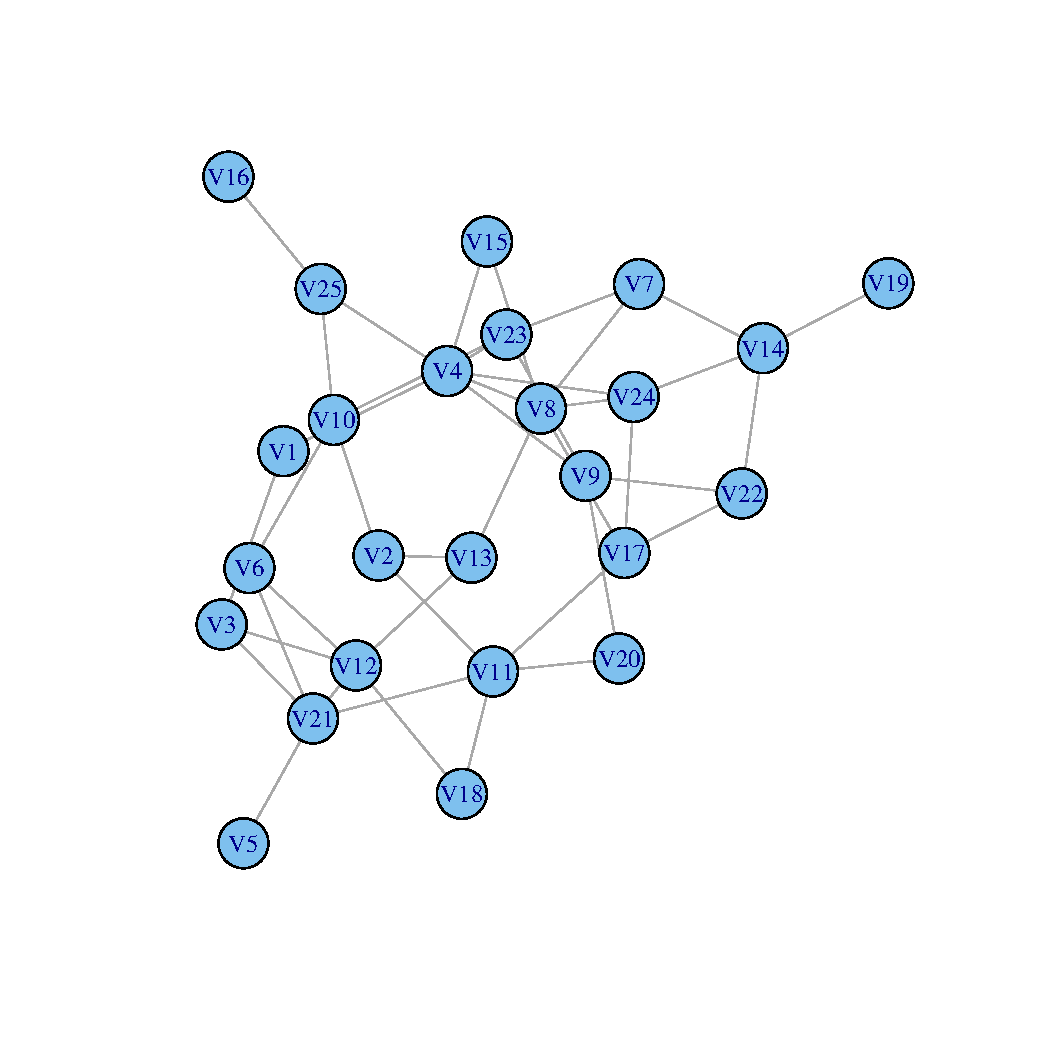
\includegraphics[scale=0.15]{Omega1hat-f.pdf}
  \caption{Estimated Nearest Neighbor Graph with Fused Lasso Penalty}
\label{fig:nearestgaphsestimate}
\end{subfigure}
\begin{subfigure}[b]{0.40\textwidth}
  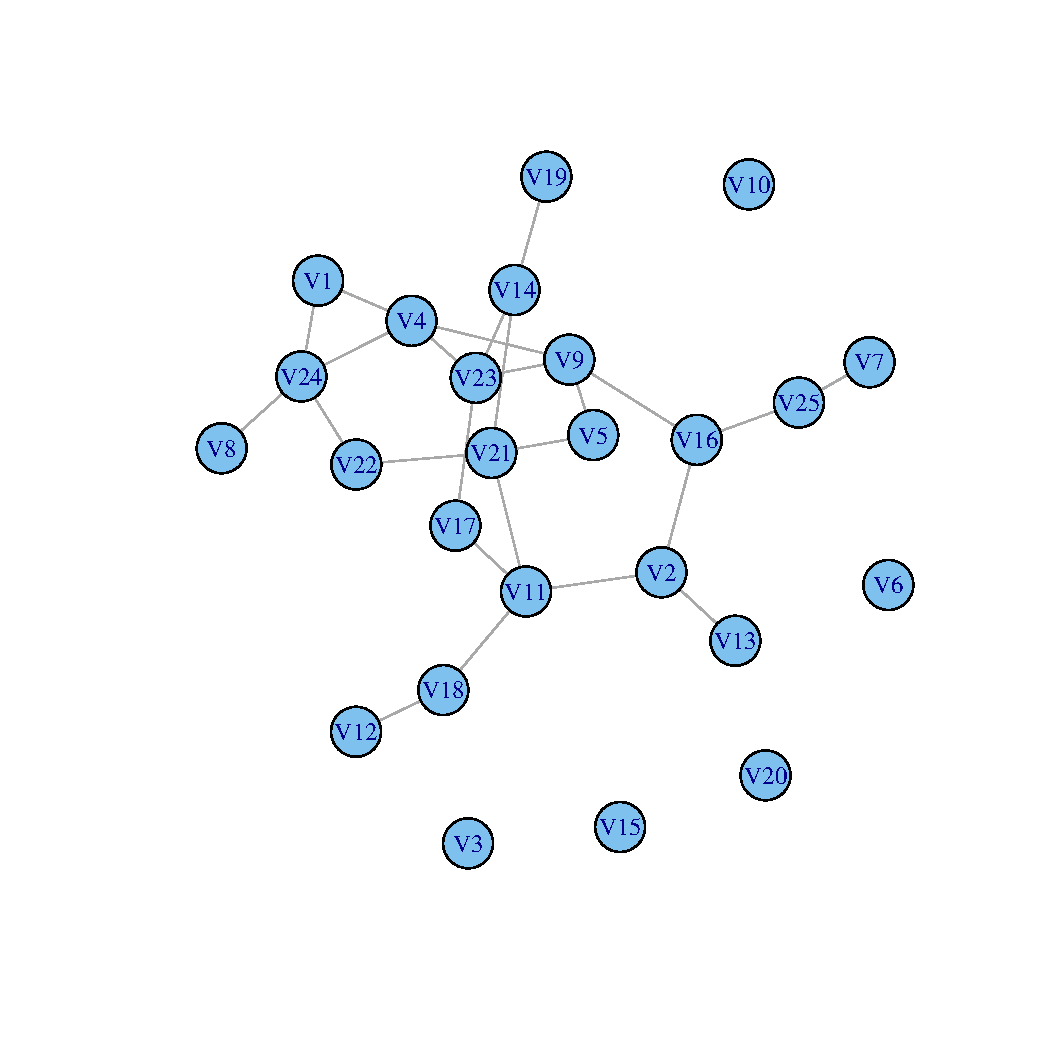
\includegraphics[scale=0.15]{Omega1hat-g.pdf}
  \caption{Estimated Nearest Neighbor Graph with Group Lasso Penalty}
\label{fig:nearestgaphsestimate}
\end{subfigure}\\
\begin{subfigure}[b]{0.50\textwidth}
  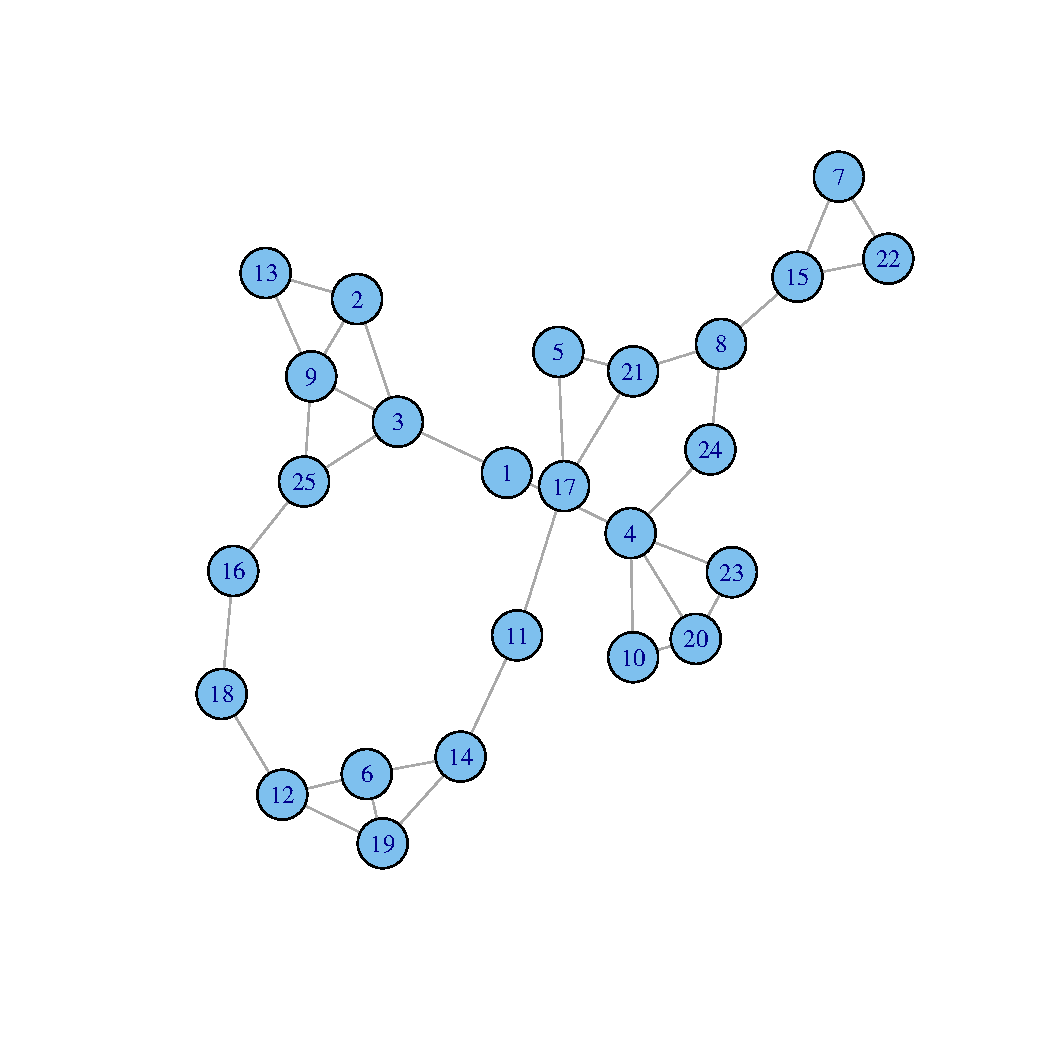
\includegraphics [scale=0.15]{Omega1-f.pdf}
  \caption{True Nearest Neighbor Graph}
\label{fig:nearestgaphsactual}
\end{subfigure}
\end{figure}
\end{frame}

\begin{frame}
\frametitle{$\hat{\Omega}_2$ for Nearest Neighbor Network (n = 100, p =25)}
\begin{figure}
\centering 
\begin{subfigure}[b]{0.40\textwidth}
  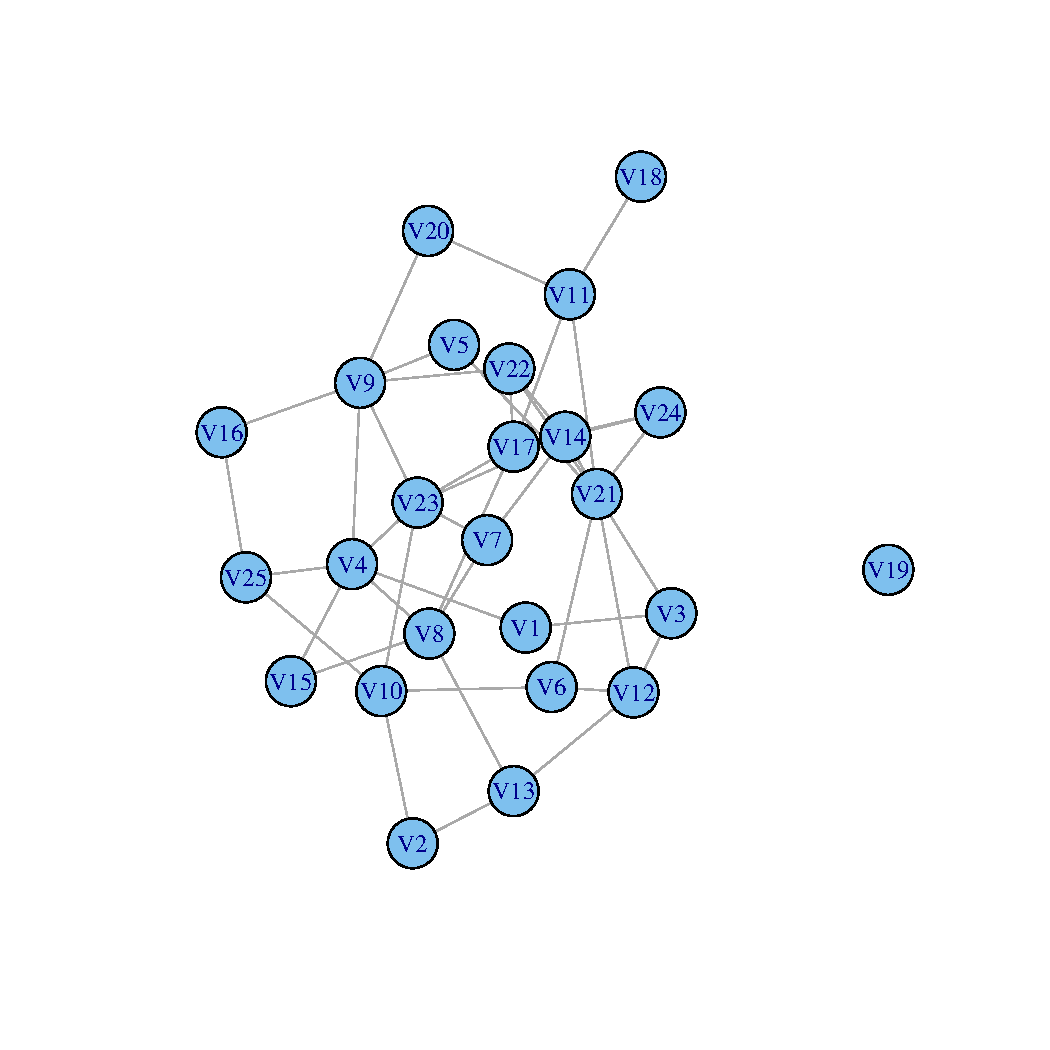
\includegraphics[scale=0.15]{Omega2hat-f.pdf}
  \caption{Estimated Nearest Neighbor Graph with Fused Lasso Penalty}
\label{fig:nearestgaphsestimate}
\end{subfigure}
\begin{subfigure}[b]{0.40\textwidth}
  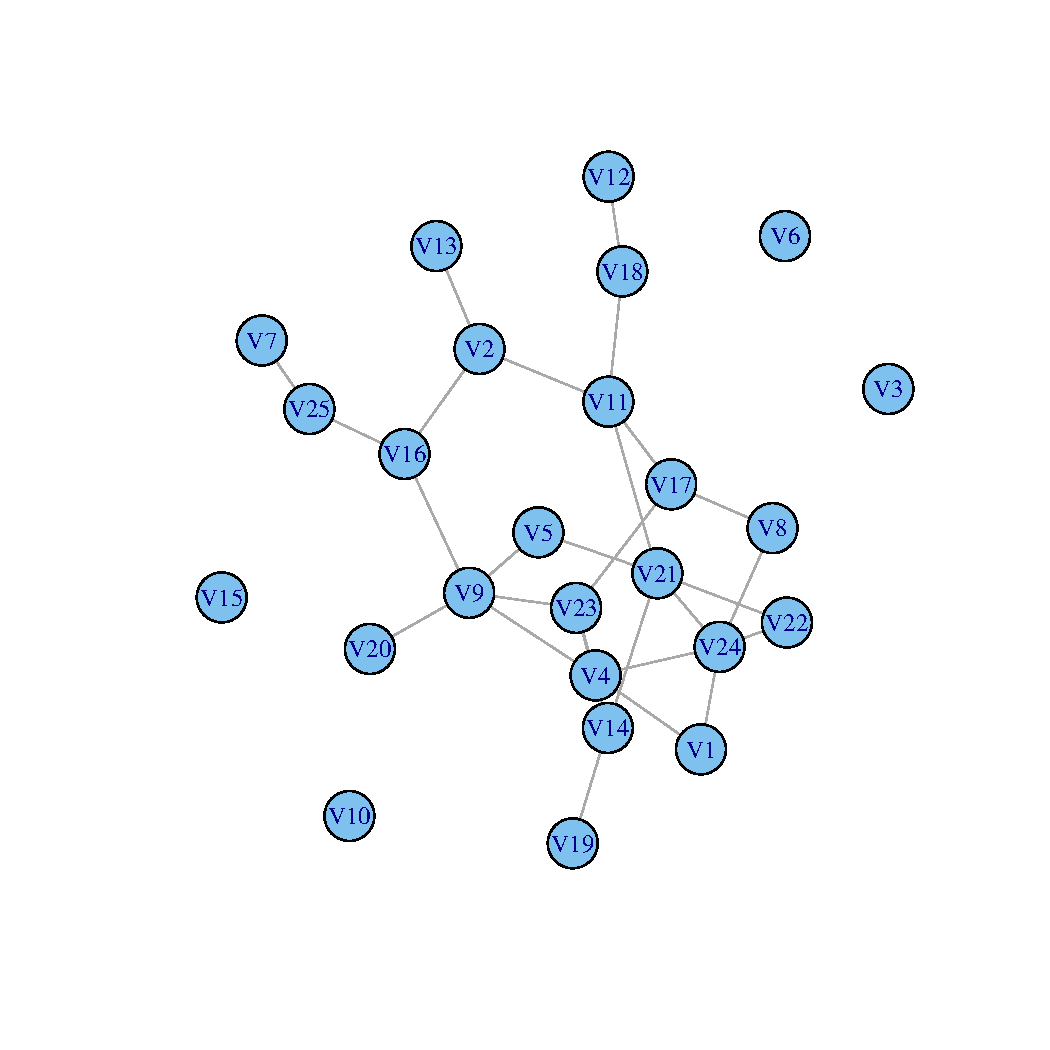
\includegraphics[scale=0.15]{Omega2hat-g.pdf}
  \caption{Estimated Nearest Neighbor Graph with Group Lasso Penalty}
\label{fig:nearestgaphsestimate}
\end{subfigure}\\
\begin{subfigure}[b]{0.50\textwidth}
  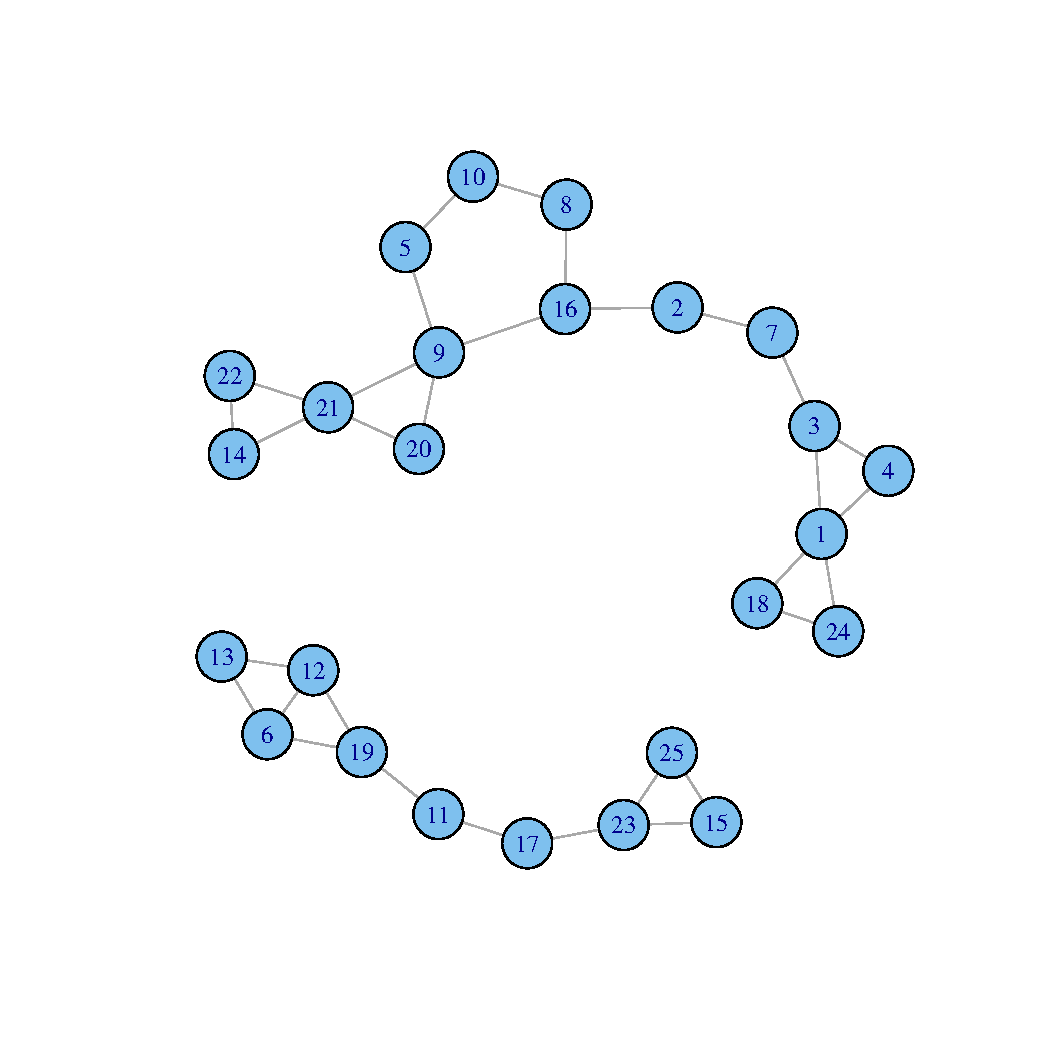
\includegraphics [scale=0.15]{Omega2-f.pdf}
  \caption{True Nearest Neighbor Graph}
\label{fig:nearestgaphsactual}
\end{subfigure}
\end{figure}
\end{frame}

\begin{frame}
\frametitle{$\hat{\Omega}_3$ for Nearest Neighbor Network (n = 100, p =25)}
\begin{figure}
\centering 
\begin{subfigure}[b]{0.40\textwidth}
  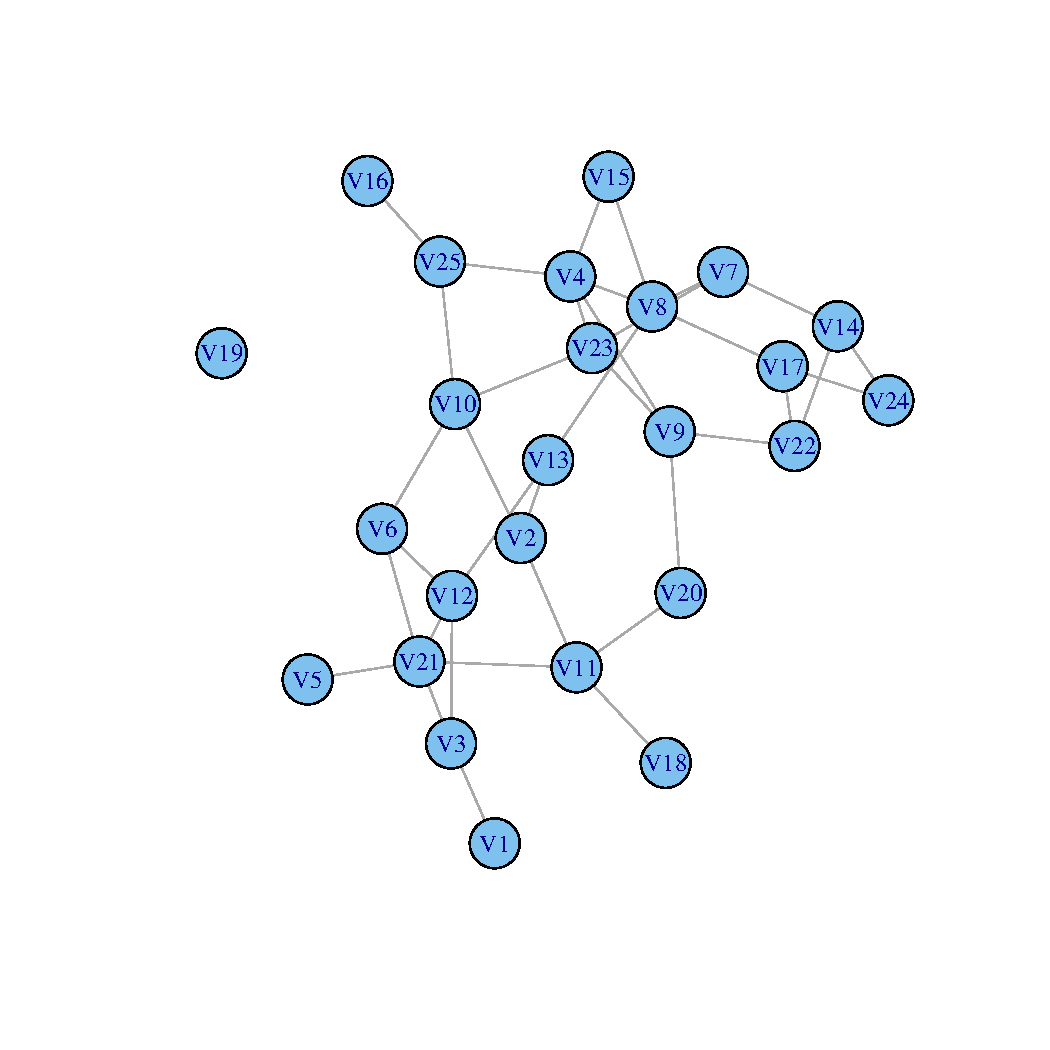
\includegraphics[scale=0.15]{Omega3hat-f.pdf}
  \caption{Estimated Nearest Neighbor Graph with Fused Lasso Penalty}
\label{fig:nearestgaphsestimate}
\end{subfigure}
\begin{subfigure}[b]{0.40\textwidth}
  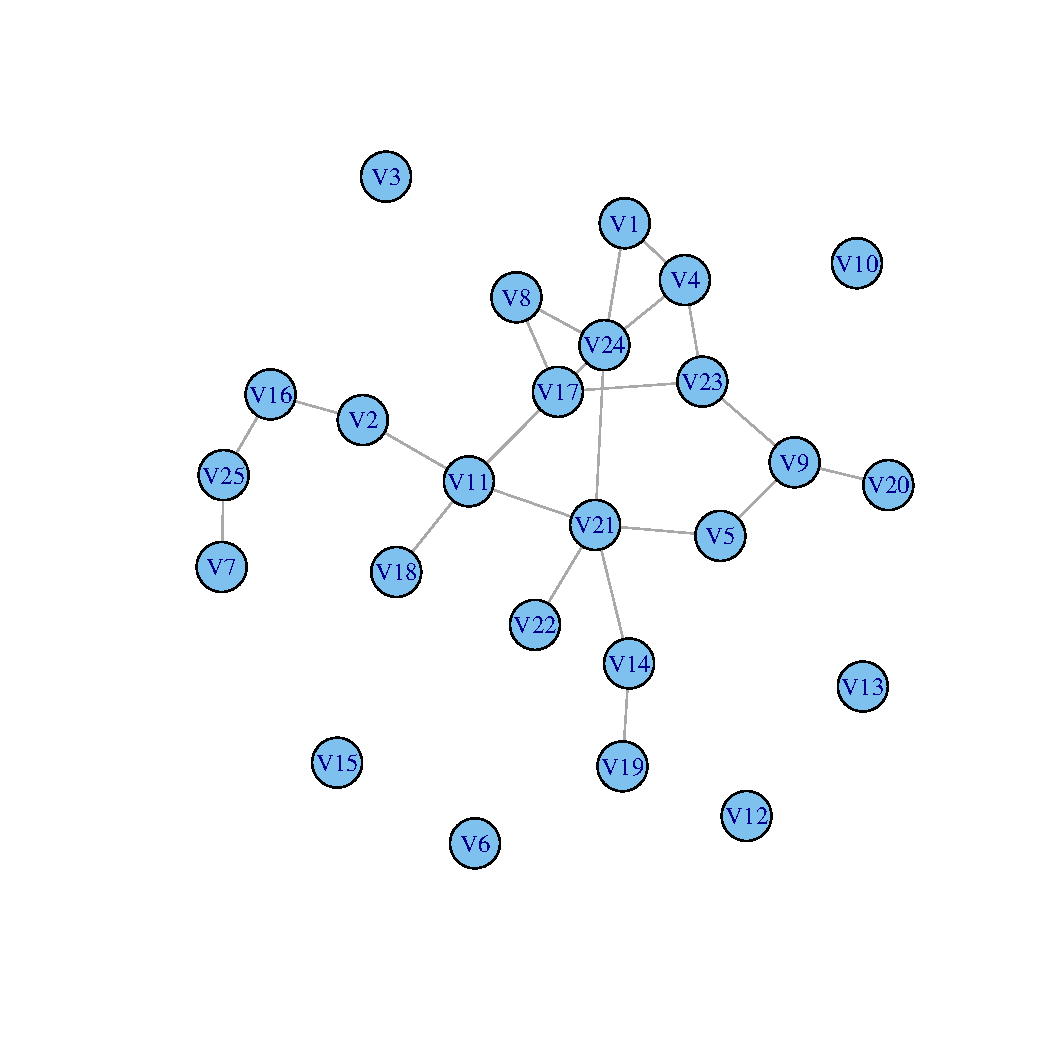
\includegraphics[scale=0.15]{Omega3hat-g.pdf}
  \caption{Estimated Nearest Neighbor Graph with Group Lasso Penalty}
\label{fig:nearestgaphsestimate}
\end{subfigure}\\
\begin{subfigure}[b]{0.50\textwidth}
  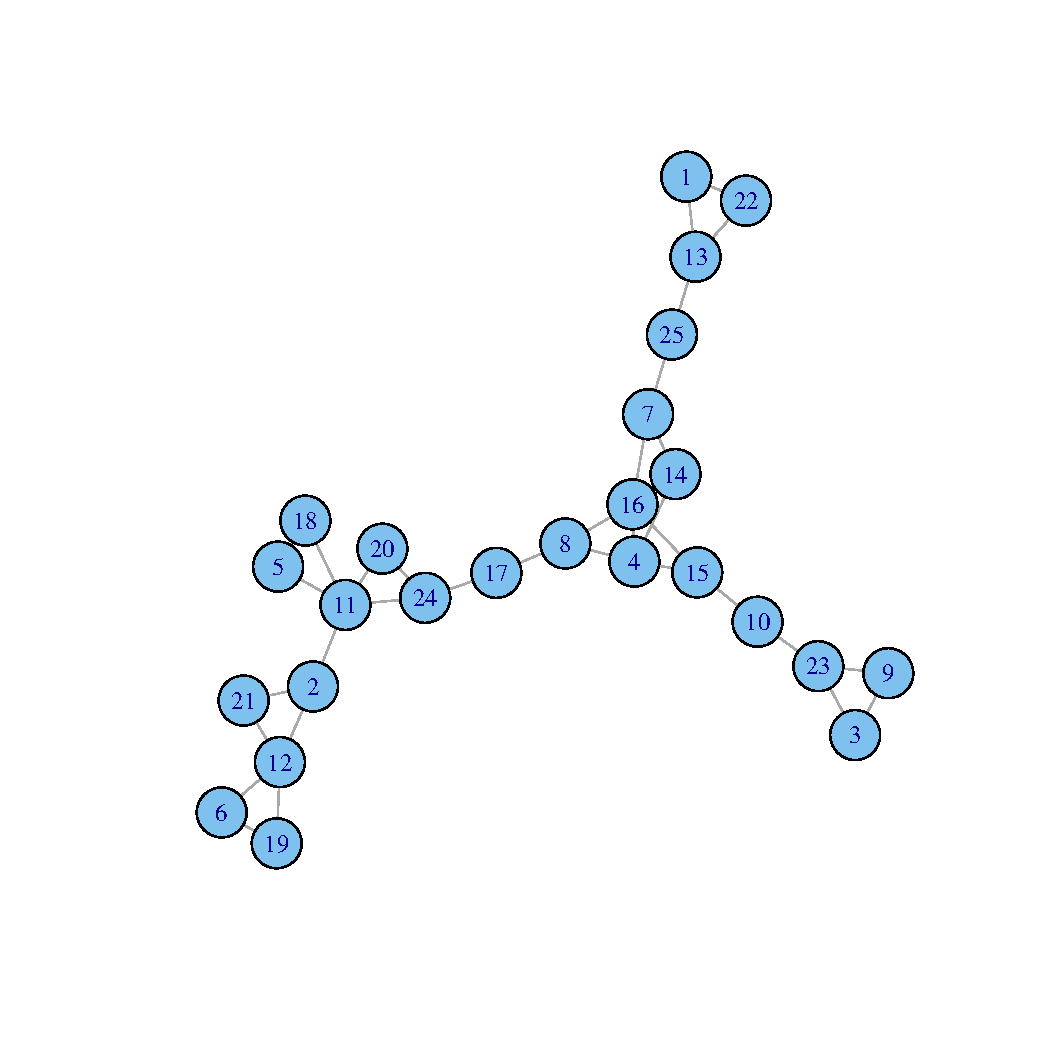
\includegraphics [scale=0.15]{Omega3-f.pdf}
  \caption{True Nearest Neighbor Graph}
\label{fig:nearestgaphsactual}
\end{subfigure}
\end{figure}
\end{frame}

\begin{frame}
\frametitle{Additional notes}
In the appendix, they show that if you go down to 2 classes, FGL performs as fast as GGL while still maintaining the results best overall.

\bigskip
\pause
We thought it was odd that the authors were much more interested in having  a low false positive rate at the cost of a high false negative instead of a balance between the two. 

\end{frame}

%\bibliographystyle{ims}
%\nocite{*}

%\begin{frame}[allowframebreaks]
%\tiny
%        \frametitle{References}
%        \bibliographystyle{amsalpha}
%        %\bibliography{../bib_files/jabrefmaster.bib}
%        \bibliography{references}
%\end{frame}
%



\end{document}

